\documentclass[10pt,a4paper,portrait]{article}

\usepackage[utf8]{inputenc}
\usepackage[a4paper,portrait,margin=0.55in,top=0.52in,bottom=0.52in]{geometry}
\usepackage{tikz}
\usetikzlibrary{shapes,arrows,positioning,calc,fit,backgrounds}
\usepackage{xcolor}
\usepackage{colortbl}
\usepackage{lmodern}
\usepackage{graphicx}
\usepackage{tabularx}
\usepackage{array}

% =========================================================
% Palette & Styling (Matching Cover 1 System)
% =========================================================
\definecolor{primary}{RGB}{20, 42, 77}        % Rich Deep Navy
\definecolor{primarylight}{RGB}{30, 64, 115}   % Medium Navy
\definecolor{secondary}{RGB}{13, 148, 136}    % Deep Cyan/Teal
\definecolor{accentgold}{RGB}{217, 119, 6}     % Warm Amber/Gold
\definecolor{darkslate}{RGB}{30, 41, 59}      % Slate 800
\definecolor{mutedgray}{RGB}{100, 116, 139}   % Slate 500
\definecolor{cardbg}{RGB}{248, 250, 252}      % Soft Light Slate 50
\definecolor{cardborder}{RGB}{226, 232, 240}  % Crisp Border Line
\definecolor{tableborder}{RGB}{215, 225, 235} % Refined Table Border

% Vertically center tabularx X columns
\renewcommand\tabularxcolumn[1]{m{#1}}

\begin{document}
\pagestyle{empty}

% =========================================================
% Subtle Minimal Outer Frame (Identical to Cover 1)
% =========================================================
\begin{tikzpicture}[remember picture, overlay]
  \draw[primary!25, line width=0.8pt, rounded corners=4pt] 
    ($(current page.north west)+(0.85cm, -0.85cm)$) rectangle ($(current page.south east)+(-0.85cm, 0.85cm)$);
\end{tikzpicture}

\vspace{0.15cm}

% =========================================================
% 1. University Logo & Department Header
% =========================================================
\begin{center}
  \IfFileExists{images/logo.png}{%
    
\includegraphics[height=1.95cm, keepaspectratio]{images/logo.png}
  }{%
    % Fallback Stylized Academic Crest
    
\begin{tikzpicture}[scale=0.80]
      \draw[primary, line width=1.5pt] (0,0) circle (1.35cm);
      \draw[secondary, line width=0.7pt, dashed] (0,0) circle (1.23cm);
      \draw[primary!30, line width=0.5pt] (0,0) circle (1.11cm);
      \fill[white] (0,0) circle (1.11cm);

      \foreach \ang in {130, 150, 170, 190, 210, 230} {
        \draw[secondary!80, fill=secondary!25, line width=0.4pt] 
          (\ang:0.90cm) ellipse (0.12cm and 0.05cm);
      }
      \foreach \ang in {50, 30, 10, -10, -30, -50} {
        \draw[secondary!80, fill=secondary!25, line width=0.4pt] 
          (\ang:0.90cm) ellipse (0.12cm and 0.05cm);
      }

      \draw[primary, fill=primary!8, line width=1.0pt, rounded corners=2pt]
        (-0.50, 0.50) -- (0.50, 0.50) -- (0.50, -0.06) arc(0:-180:0.50cm) -- cycle;
      
      \draw[primary, line width=1.0pt] (0, 0.42) -- (0, -0.36);
      \draw[secondary, line width=0.8pt] (-0.36, 0.28) to[bend left=15] (-0.06, 0.28);
      \draw[secondary, line width=0.8pt] (-0.36, 0.10) to[bend left=15] (-0.06, 0.10);
      \draw[secondary, line width=0.8pt] (-0.36, -0.08) to[bend left=15] (-0.06, -0.08);
      \draw[secondary, line width=0.8pt] (0.36, 0.28) to[bend right=15] (0.06, 0.28);
      \draw[secondary, line width=0.8pt] (0.36, 0.10) to[bend right=15] (0.06, 0.10);
      \draw[secondary, line width=0.8pt] (0.36, -0.08) to[bend right=15] (0.06, -0.08);

      \node[accentgold, font=\small] at (0, 0.72) {$\star$};
      \node[primary, font=\fontsize{4.5}{5.2}\selectfont\bfseries\sffamily] at (0, -0.76) {ESTD 2012};
    \end{tikzpicture}
  }

  \vspace{0.14cm}
  {\fontsize{18}{22}\selectfont\bfseries\sffamily\color{primary} KHWAJA YUNUS ALI UNIVERSITY\par}
  \vspace{0.05cm}
  {\fontsize{9.5}{12}\selectfont\bfseries\sffamily\color{secondary} DEPARTMENT OF COMPUTER SCIENCE AND ENGINEERING\par}
  
  \vspace{0.12cm}
  % Sleek Minimal Divider Line with Center Diamond
  
\begin{tikzpicture}
    \draw[primary!20, line width=0.6pt] (-4.5, 0) -- (4.5, 0);
    \draw[secondary, line width=1.4pt] (-1.8, 0) -- (1.8, 0);
    \draw[fill=primary, rotate=45] (-0.065, -0.065) rectangle (0.065, 0.065);
  \end{tikzpicture}
\end{center}

\vspace{0.12cm}

% =========================================================
% 2. Laboratory Report Index Badge & Course Info
% =========================================================
\begin{center}
  
\begin{tikzpicture}
    \node[
      fill=primary,
      text=white,
      font=\fontsize{10.5}{12.5}\selectfont\bfseries\sffamily,
      inner xsep=20pt,
      inner ysep=4.5pt,
      rounded corners=3pt
    ] {LABORATORY REPORT INDEX};
  \end{tikzpicture}

  \vspace{0.14cm}
  
\begin{tikzpicture}
    \node[
      draw=primary!20,
      fill=white,
      rounded corners=5pt,
      line width=0.65pt,
      inner xsep=18pt,
      inner ysep=5.5pt
    ] {
      \sffamily
      \textbf{\color{mutedgray}\small COURSE:} \textbf{\normalsize\color{primary} Operating System Lab} \quad
      \textcolor{primary!30}{\textbf{\textbar}} \quad
      \textbf{\color{mutedgray}\small CODE:} \textbf{\normalsize\color{secondary} CSE 0613-3104}
    };
  \end{tikzpicture}
\end{center}

\vspace{0.18cm}

% =========================================================
% 3. Index of Experiments Table (3 Columns, 17 Rows)
% =========================================================
\begin{center}
{\renewcommand{\arraystretch}{1.34}%
\setlength{\arrayrulewidth}{0.5pt}%
\arrayrulecolor{tableborder}%
\begin{tabularx}{\linewidth}{|>{\centering\arraybackslash}m{1.6cm}|>{\raggedright\arraybackslash}X|>{\centering\arraybackslash}m{1.5cm}|}
\hline
\rowcolor{primary}
\textbf{\color{white}\sffamily\footnotesize Lab No.} & 
\textbf{\color{white}\sffamily\footnotesize Title of the Experiment} & 
\textbf{\color{white}\sffamily\footnotesize Page} \\
\hline
\rowcolor{white}
{\color{primary}\sffamily\bfseries\footnotesize 01} & {\sffamily\footnotesize\color{darkslate} Installation and Configuration of Linux Operating System} & \\
\hline
\rowcolor{cardbg}
{\color{primary}\sffamily\bfseries\footnotesize 02} & {\sffamily\footnotesize\color{darkslate} Practice of Basic Linux Terminal Commands} & \\
\hline
\rowcolor{white}
{\color{primary}\sffamily\bfseries\footnotesize 03} & {\sffamily\footnotesize\color{darkslate} File and Directory Management in Linux Terminal} & \\
\hline
\rowcolor{cardbg}
{\color{primary}\sffamily\bfseries\footnotesize 04} & {\sffamily\footnotesize\color{darkslate} Viewing and Editing Files in Linux Terminal} & \\
\hline
\rowcolor{white}
{\color{primary}\sffamily\bfseries\footnotesize 05} & {\sffamily\footnotesize\color{darkslate} Searching Files and Content in Linux Terminal} & \\
\hline
\rowcolor{cardbg}
{\color{primary}\sffamily\bfseries\footnotesize 06} & {\sffamily\footnotesize\color{darkslate} Package Management in Linux (Debian/Ubuntu)} & \\
\hline
\rowcolor{white}
{\color{primary}\sffamily\bfseries\footnotesize 07} & {\sffamily\footnotesize\color{darkslate} Helpful Utilities in Linux Terminal} & \\
\hline
\rowcolor{cardbg}
{\color{primary}\sffamily\bfseries\footnotesize 08} & {\sffamily\footnotesize\color{darkslate} Implementation of First Come, First Served CPU Scheduling Algorithm in C++} & \\
\hline
\rowcolor{white}
{\color{primary}\sffamily\bfseries\footnotesize 09} & {\sffamily\footnotesize\color{darkslate} Implementation of Shortest Job First (SJF) Non-Preemptive CPU Scheduling Algorithm} & \\
\hline
\rowcolor{cardbg}
{\color{primary}\sffamily\bfseries\footnotesize 10} & {\sffamily\footnotesize\color{darkslate} Implementation of Shortest Remaining Job First (SRJF) CPU Scheduling Algorithm} & \\
\hline
\rowcolor{white}
{\color{mutedgray}\sffamily\footnotesize 11} & & \\
\hline
\rowcolor{cardbg}
{\color{mutedgray}\sffamily\footnotesize 12} & & \\
\hline
\rowcolor{white}
{\color{mutedgray}\sffamily\footnotesize 13} & & \\
\hline
\rowcolor{cardbg}
{\color{mutedgray}\sffamily\footnotesize 14} & & \\
\hline
\rowcolor{white}
{\color{mutedgray}\sffamily\footnotesize 15} & & \\
\hline
\rowcolor{cardbg}
{\color{mutedgray}\sffamily\footnotesize 16} & & \\
\hline
\rowcolor{white}
{\color{mutedgray}\sffamily\footnotesize 17} & & \\
\hline
\end{tabularx}%
}
\end{center}

\vspace{0.20cm}

% =========================================================
% 4. Submitted By & Submitted To Cards
% =========================================================
\begin{center}
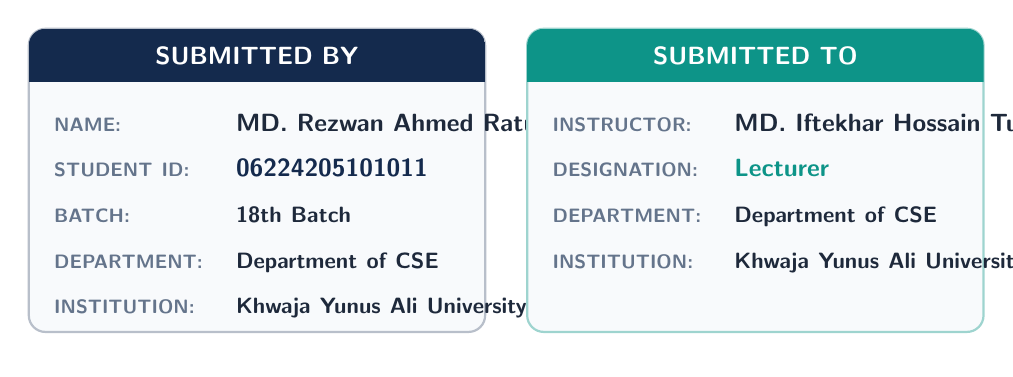
\begin{tikzpicture}
  % Dimensions
  \def\cardw{0.478\linewidth}
  \def\cardh{3.85cm}
  \def\headerh{0.68cm}

  % Card Left: Submitted By
  \coordinate (cl_topleft) at (0, 0);
  \coordinate (cl_botright) at (\cardw, -\cardh);
  
  \fill[cardbg, rounded corners=6pt] (cl_topleft) rectangle (cl_botright);
  \draw[primary!30, line width=0.8pt, rounded corners=6pt] (cl_topleft) rectangle (cl_botright);
  
  % Header Left
  \begin{scope}
    \clip[rounded corners=6pt] (cl_topleft) rectangle (cl_botright);
    \fill[primary] (cl_topleft) rectangle ($(cl_topleft)+(\cardw, -\headerh)$);
  \end{scope}
  \node[text=white, font=\sffamily\bfseries\small, anchor=center] at ($(cl_topleft)+(0.5*\cardw, -0.5*\headerh)$) {SUBMITTED BY};

  % Content Left (Structured Table)
  \node[anchor=north west, inner sep=9pt, text width=\dimexpr\cardw-18pt\relax] at ($(cl_topleft)+(0, -\headerh)$) {
    \vspace{-1pt}
    \begin{tabular}{@{}ll@{}}
      \sffamily\fontsize{7.5}{9.5}\selectfont\textbf{\color{mutedgray}NAME:} & 
      \sffamily\bfseries\fontsize{9}{11.5}\selectfont\color{darkslate} MD. Rezwan Ahmed Ratul\\[4.5pt]
      \sffamily\fontsize{7.5}{9.5}\selectfont\textbf{\color{mutedgray}STUDENT ID:} & 
      \sffamily\bfseries\fontsize{9}{11.5}\selectfont\color{primary} 06224205101011\\[4.5pt]
      \sffamily\fontsize{7.5}{9.5}\selectfont\textbf{\color{mutedgray}BATCH:} & 
      \sffamily\bfseries\fontsize{8.5}{11}\selectfont\color{darkslate} 18th Batch\\[4.5pt]
      \sffamily\fontsize{7.5}{9.5}\selectfont\textbf{\color{mutedgray}DEPARTMENT:} & 
      \sffamily\bfseries\fontsize{8.5}{11}\selectfont\color{darkslate} Department of CSE\\[4.5pt]
      \sffamily\fontsize{7.5}{9.5}\selectfont\textbf{\color{mutedgray}INSTITUTION:} & 
      \sffamily\bfseries\fontsize{8.5}{11}\selectfont\color{darkslate} Khwaja Yunus Ali University
    \end{tabular}
  };

  % Card Right: Submitted To
  \coordinate (cr_topleft) at (0.522\linewidth, 0);
  \coordinate (cr_botright) at ($(cr_topleft)+(\cardw, -\cardh)$);
  
  \fill[cardbg, rounded corners=6pt] (cr_topleft) rectangle (cr_botright);
  \draw[secondary!40, line width=0.8pt, rounded corners=6pt] (cr_topleft) rectangle (cr_botright);
  
  % Header Right
  \begin{scope}
    \clip[rounded corners=6pt] (cr_topleft) rectangle (cr_botright);
    \fill[secondary] (cr_topleft) rectangle ($(cr_topleft)+(\cardw, -\headerh)$);
  \end{scope}
  \node[text=white, font=\sffamily\bfseries\small, anchor=center] at ($(cr_topleft)+(0.5*\cardw, -0.5*\headerh)$) {SUBMITTED TO};

  % Content Right (Structured Table)
  \node[anchor=north west, inner sep=9pt, text width=\dimexpr\cardw-18pt\relax] at ($(cr_topleft)+(0, -\headerh)$) {
    \vspace{-1pt}
    \begin{tabular}{@{}ll@{}}
      \sffamily\fontsize{7.5}{9.5}\selectfont\textbf{\color{mutedgray}INSTRUCTOR:} & 
      \sffamily\bfseries\fontsize{9}{11.5}\selectfont\color{darkslate} MD. Iftekhar Hossain Tushar\\[4.5pt]
      \sffamily\fontsize{7.5}{9.5}\selectfont\textbf{\color{mutedgray}DESIGNATION:} & 
      \sffamily\bfseries\fontsize{9}{11.5}\selectfont\color{secondary} Lecturer\\[4.5pt]
      \sffamily\fontsize{7.5}{9.5}\selectfont\textbf{\color{mutedgray}DEPARTMENT:} & 
      \sffamily\bfseries\fontsize{8.5}{11}\selectfont\color{darkslate} Department of CSE\\[4.5pt]
      \sffamily\fontsize{7.5}{9.5}\selectfont\textbf{\color{mutedgray}INSTITUTION:} & 
      \sffamily\bfseries\fontsize{8.5}{11}\selectfont\color{darkslate} Khwaja Yunus Ali University
    \end{tabular}
  };
\end{tikzpicture}
\end{center}

\vfill

% =========================================================
% 5. Instructor's Signature & Evaluation Box
% =========================================================
\begin{center}

\begin{tikzpicture}
  \node[
    draw=primary!20,
    line width=0.7pt,
    fill=white,
    rounded corners=5pt,
    inner xsep=16pt,
    inner ysep=11pt,
    text width=\dimexpr\linewidth-32pt-2pt\relax
  ] {
    \begin{tabular*}{\linewidth}{@{\extracolsep{\fill}}lr@{}}
      \begin{tabular}{@{}l@{}}
        \textbf{\sffamily\small\color{darkslate} Remarks / Evaluation:}\\[14pt]
        \rule{5.2cm}{0.4pt}
      \end{tabular} &
      \begin{tabular}{@{}c@{}}
        \vspace{14pt}\null\\
        \rule{5.6cm}{0.5pt}\\[3pt]
        \textbf{\sffamily\small\color{primary} Instructor's Signature \& Date}
      \end{tabular}
    \end{tabular*}
  };
\end{tikzpicture}
\end{center}

\vspace{0.25cm}

\end{document}
